\chapter{Finanzen}
\label{chap:finanzen}

\section{Finanzierungskonzept}
Unser Unternehmen wird mit diesem Projekt gegr\"undet. Durch Crowdfunding kann man auf einfache Weise erfahren, ob ein Produkt f\"ur potentielle Kunden attraktiv ist oder nicht. Die Finanzierung des Projekts wird in diesem Fall haupts�chlich �ber Darlehen dritter (Backer) sichergestellt. Bei den meisten Crowdfundingplatformen muss man einen Kapitalbedarf angeben (Goal), der die Realisierung des Projekts erm\"oglicht. Wenn der Kapitalbedarf innerhalb von 30 Tagen erreicht wird, kann das Unternehmen dieses Geld fordern und die Produktion beginnen. Innerhalb von drei Jahren sollten dann alle Produkte geliefert werden. Das Unternehmen braucht momentan keine Werbung, weil die Kunden durch Crowdfunding gesucht werden.

\subsection{Rahmenbedingungen}

\paragraph{Anzahl Kunden} Wir haben die Anzahl Kunden an der durchschnittlichen Anzahl Kunden von anderer \"ahnlichen Projekten abgesch\"atzt. Einige Projekte im IT Bereich erhalten bis zu 16000 Kunden oder Backers. 

\paragraph{Anzahl Kunden} Wir haben die Anzahl Kunden an der durchschnittlichen Anzahl Kunden von anderer \"ahnlichen Projekten abgesch\"atzt. Einige Projekte im IT Bereich erhalten bis zu 16000 Kunden oder Backers. 

\paragraph{Gewinn} Wir rechnen mit einem EBT von 10'000 CHF pro Jahr.

\paragraph{Material und Produktion} Wir haben die Materialkosten pro St\"uck auf CHF 10.- gesch\"atzt, und die Produktionskosten (Strom, Verpackung, usw.) auf CHF 2.- .

\subsection{Weitere Kostenpunkte}

\paragraph{L\"ohne} Unser Team besteht aus 6 Personen. \\
\begin{table}[H]
\begin{tabular}{lll}
\textbf{Position} & \textbf{Monatsgehalt}  \\ \hline
  \textbf{CEO} &  CHF 4700.- \\ \hline
 \textbf{CFO} &  CHF 4700.- \\ \hline
 \textbf{Technischer Direktor}& CHF 4700.-  \\ \hline
 \textbf{Mitarbeiter} &CHF  3500.- \\ \hline
 \textbf{Durchschnitt} & CHF 4000.-\\ \hline
\end{tabular}
\centering
\caption{L\"ohne}
\label{L\"ohne}
\end{table}

\paragraph{Webserver} Um unser Produkt zu vermarkten und den Kontakt zu unseren Kunden zu pflegen.

\paragraph{Crowdfundinggeb�hren} Webseiten wie Kickstarter und Indiegogo verlangen einen Anteil von 10\% des Goals, falls das Goal erreicht wird.

\paragraph{Mietzins} 700.- CHF pro Monat

\paragraph{Copyright} 100.- CHF

\paragraph{Abschreibungen} wir buchen Abschreibungen auf Produktionsmaschinen und sonstigem (Ankauf 5000.- CHF), in der h\"ohe von 10\% pro Jahr (angenommene Lebensdauer: 10 Jahre).
\paragraph{Analyse und Marketing} Anfangsstudien die vor dem Crowdfunding gemacht wurden.

\section{Steuern}
Als Referenzort f�r die Steuerberechnung nehmen wir Deisswil bei M\"unchenbuchsee. Dort  muss ein Gewinn von 10'000 CHF mit 3'966.- CHF versteuert werden.

\section{Zukunft}
Wir haben die Finanzplanung f\"ur die ersten 3 Jahre erstellt. Innerhalb dieser 3 Jahre werden wir den Backers das Produkt liefern. Falls die Nachfrage vorhanden ist, planen wir eine neue Version des Smoilet Produkts in den folgenden Jahren herzustellen. 

\section{Kosten\"ubersicht}
Die nachfolgenden Tabellen illustrieren die zu erwartenden variablen und fixen Kosten. Die Fixkosten nehmen im Verlauf der weiteren Jahre ab, da z.Bsp. die Analyse und Marketing Kosten nur im ersten Jahr anfallen.

\begin{landscape}

\begin{figure}[H]
	\minipage{0.32\textwidth}
		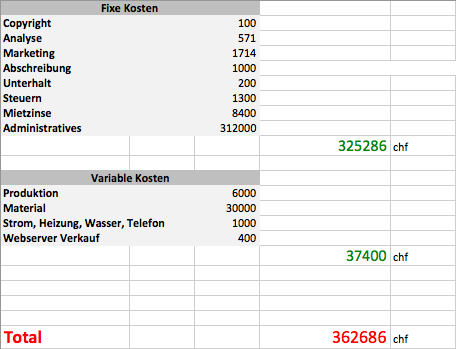
\includegraphics[scale=0.48]{bilder/Jahr1.png}
	\caption{erstes Jahr}
	\label{fig:Jahr1}
	\endminipage\hfill
	\minipage{0.32\textwidth}
		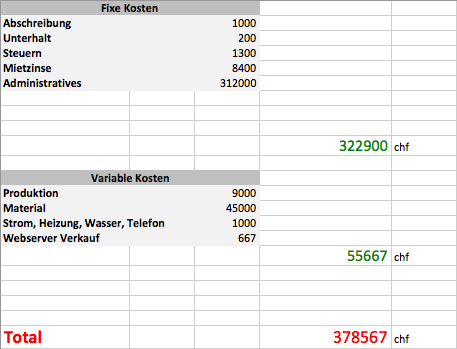
\includegraphics[scale=0.48]{bilder/Jahr2.png}
	\caption{zweites Jahr}
	\label{fig:Jahr2}
	\endminipage\hfill
	\minipage{0.32\textwidth}
		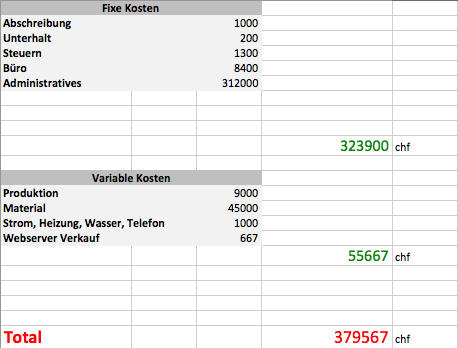
\includegraphics[scale=0.48]{bilder/Jahr3.png}
	\caption{drittes Jahr}
	\label{fig:Jahr3}
	\endminipage\hfill
\end{figure}

\begin{figure}[H]
	\centering
	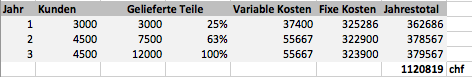
\includegraphics[scale=0.48]{bilder/kosten_ubersicht.png}
	\caption{Jahrestotal}
	\label{fig:Jahrestotal}
\end{figure}

\end{landscape}

\begin{figure}[H]
	\centering
	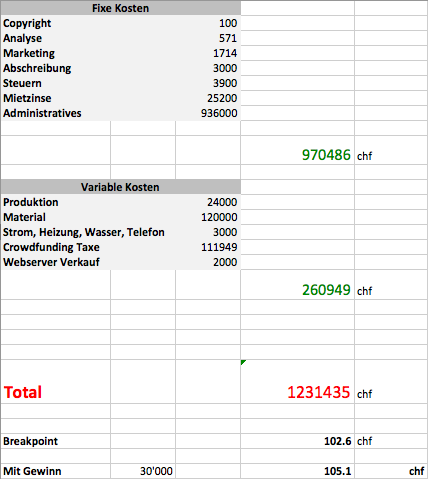
\includegraphics[scale=0.6]{bilder/3Jahre.png}
	\caption{Kosten\"ubersicht 3 Jahre}
	\label{fig:3Jahre}
\end{figure}

\section{Kapitalbedarf}
Eine Vollkostendeckung f�r sechs Ingenieurl�hne ist in den ersten drei Jahren nicht realistisch. Nachfolgend wollen wir zwei Strategien aufzeigen um diese Problematik zu entsch�rfen.

\subsection{Startfinanzierung durch Investoren}
Wir haben die Suche nach einem Investor die die Grundkosten der Firma beim Startup finanzieren w\"urden auf Firmen im Umfeld der Sanit\"artechnik beschr\"ankt:
\begin{itemize}
\item Geberit
\item Cera
\item Kohler
\item Das Bad
\item B+R Sanit\"arcenter AG
\end{itemize}
Mit einer Finanzierung von 1'000'000.- CHF k\"onnten wir drei Jahre lang unsere L\"ohne bezahlen. W\"ahrend diesen drei Jahren erstellen wir Smoilet 2.0 Prototype, testen Produktionsverbesserungen aus und werten Kundenfeedback aus. Das Finale Produkt wird dann im Rahmen der Crowdfundingkampagne an den Markt gebracht. Die Finanzierungen k\"onnten wir dann mit dem Gewinn der folgenden Jahren zur\"uckbezahlen. 

Das Geld der Crowdfundingkampagne wird verwendet um die Produktion der einzelnen Teile zu decken. Weiter ist die Kampagne eine ideale Werbeplattform. Wenn kein Investor an unserem Produkt interessiert ist, bewerben wir uns bei \textit{SharkTank}, eine Reality-Show f�r Investoren und Unternehmer. Mit ein bisschen Gl\"uck k\"onnten wir dort eine interessante Gelegenheit finden.

\subsection{Ehramtliche Arbeit}
Arbeiten wir ausschliesslich ehrenamtlich, kann f�r ein St�ckpreis von 39.90 CHF der Gewinn auf 185'000 CHF maximiert werden.
\begin{figure}[H]
	\centering
		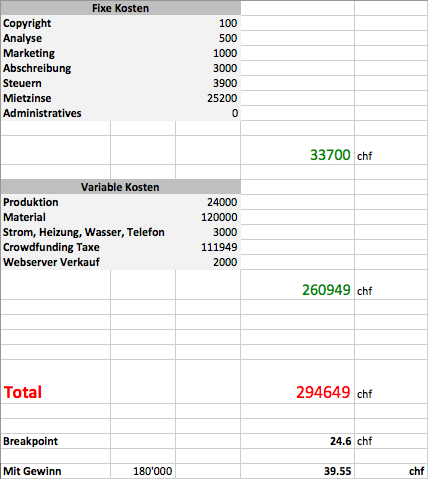
\includegraphics[scale=0.6]{bilder/ehramtlich.png}
	\caption{Kosten\"ubersicht ohne Ingenieurl\"ohne}
	\label{fig:ehramtlich}
\end{figure}
Die Steuern f\"ur einen Gewinn von 185'000.- CHF pro Jahr betragen in Deisswil bei M\"unchenbuchsee 24'460.- CHF im Jahr.

\section{Fazit}
Um den Finanzteil mit einer realistischen Planerfolgsrechnung abzuschliessen, w\"aren wir auf genaue Angaben \"uber Kosten angewiesen. Leider ist es im Rahmen dieser Arbeit nahezu unm\"oglich, an diese Zahlen zu gelangen. Ziel des Crowdfundings liegt nicht prim\"ar in der Umsatzsteigerung, sondern in der Gewinnmaximierung durch Kostenersparnisse in Bezug auf Werbung und Kundensuche. 